% Created by tikzDevice version 0.10.1 on 2016-09-19 13:44:36
% !TEX encoding = UTF-8 Unicode
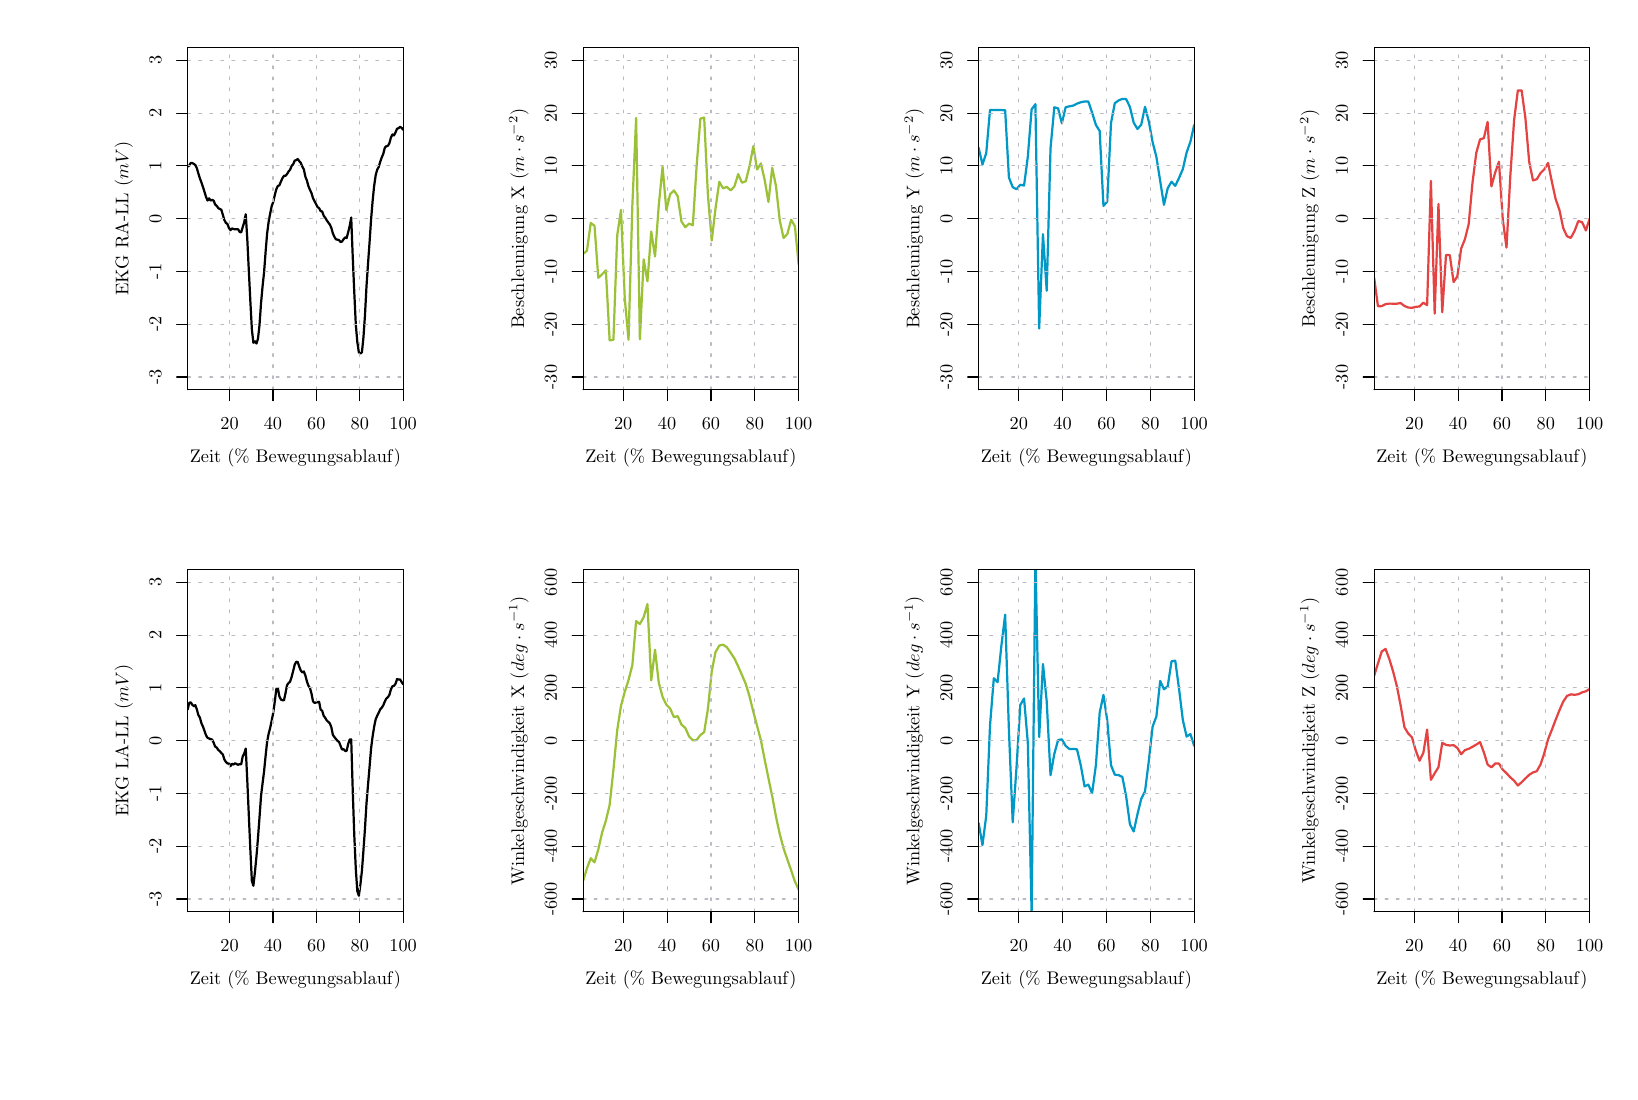
\begin{tikzpicture}[x=1pt,y=1pt]
\definecolor{fillColor}{RGB}{255,255,255}
\path[use as bounding box,fill=fillColor] (0,0) rectangle (571.66,377.25);
\begin{scope}
\path[clip] ( 57.82,246.44) rectangle (135.69,370.02);
\definecolor{drawColor}{RGB}{0,0,0}

\path[draw=drawColor,line width= 0.8pt,line join=round,line cap=round] ( 57.82,327.07) --
	( 58.37,327.42) --
	( 58.92,328.37) --
	( 59.47,328.34) --
	( 60.03,328.02) --
	( 60.58,327.61) --
	( 61.13,326.47) --
	( 61.68,324.55) --
	( 62.23,322.80) --
	( 62.79,321.29) --
	( 63.34,319.69) --
	( 63.89,317.94) --
	( 64.44,316.10) --
	( 65.00,314.78) --
	( 65.55,315.58) --
	( 66.10,314.77) --
	( 66.65,315.02) --
	( 67.20,314.76) --
	( 67.76,313.33) --
	( 68.31,312.86) --
	( 68.86,312.06) --
	( 69.41,311.74) --
	( 69.97,311.49) --
	( 70.52,309.65) --
	( 71.07,307.74) --
	( 71.62,306.71) --
	( 72.18,306.31) --
	( 72.73,304.87) --
	( 73.28,304.08) --
	( 73.83,304.72) --
	( 74.38,304.48) --
	( 74.94,304.40) --
	( 75.49,304.40) --
	( 76.04,304.40) --
	( 76.59,303.44) --
	( 77.15,303.28) --
	( 77.70,305.19) --
	( 78.25,306.94) --
	( 78.80,309.84) --
	( 79.35,300.97) --
	( 79.91,289.48) --
	( 80.46,278.47) --
	( 81.01,268.23) --
	( 81.56,263.38) --
	( 82.12,263.92) --
	( 82.67,263.13) --
	( 83.22,264.83) --
	( 83.77,269.81) --
	( 84.33,277.78) --
	( 84.88,283.80) --
	( 85.43,288.96) --
	( 85.98,296.28) --
	( 86.53,302.94) --
	( 87.09,307.21) --
	( 87.64,310.17) --
	( 88.19,312.82) --
	( 88.74,314.26) --
	( 89.30,316.79) --
	( 89.85,318.89) --
	( 90.40,320.04) --
	( 90.95,320.27) --
	( 91.50,321.60) --
	( 92.06,322.89) --
	( 92.61,323.71) --
	( 93.16,323.72) --
	( 93.71,324.33) --
	( 94.27,325.29) --
	( 94.82,325.92) --
	( 95.37,327.28) --
	( 95.92,327.84) --
	( 96.48,329.20) --
	( 97.03,329.38) --
	( 97.58,329.79) --
	( 98.13,329.02) --
	( 98.68,328.39) --
	( 99.24,327.04) --
	( 99.79,326.04) --
	(100.34,323.42) --
	(100.89,322.03) --
	(101.45,319.98) --
	(102.00,318.66) --
	(102.55,317.49) --
	(103.10,315.65) --
	(103.65,314.58) --
	(104.21,313.48) --
	(104.76,312.41) --
	(105.31,312.02) --
	(105.86,310.98) --
	(106.42,310.83) --
	(106.97,309.27) --
	(107.52,308.58) --
	(108.07,307.65) --
	(108.63,306.83) --
	(109.18,306.13) --
	(109.73,304.91) --
	(110.28,302.91) --
	(110.83,301.67) --
	(111.39,300.76) --
	(111.94,300.64) --
	(112.49,300.52) --
	(113.04,299.80) --
	(113.60,299.96) --
	(114.15,300.82) --
	(114.70,301.45) --
	(115.25,301.22) --
	(115.80,303.29) --
	(116.36,305.59) --
	(116.91,308.64) --
	(117.46,294.43) --
	(118.01,281.80) --
	(118.57,269.92) --
	(119.12,263.62) --
	(119.67,259.93) --
	(120.22,259.45) --
	(120.78,259.95) --
	(121.33,265.34) --
	(121.88,273.27) --
	(122.43,283.79) --
	(122.98,291.89) --
	(123.54,299.70) --
	(124.09,307.90) --
	(124.64,314.58) --
	(125.19,320.03) --
	(125.75,323.95) --
	(126.30,325.93) --
	(126.85,326.95) --
	(127.40,328.81) --
	(127.96,330.39) --
	(128.51,331.69) --
	(129.06,333.87) --
	(129.61,334.43) --
	(130.16,334.53) --
	(130.72,335.53) --
	(131.27,337.59) --
	(131.82,338.65) --
	(132.37,338.31) --
	(132.93,339.44) --
	(133.48,340.74) --
	(134.03,340.94) --
	(134.58,341.42) --
	(135.13,341.04) --
	(135.69,340.33);
\end{scope}
\begin{scope}
\path[clip] (  0.00,  0.00) rectangle (571.66,377.25);
\definecolor{drawColor}{RGB}{0,0,0}

\path[draw=drawColor,line width= 0.4pt,line join=round,line cap=round] ( 72.95,246.44) -- (135.69,246.44);

\path[draw=drawColor,line width= 0.4pt,line join=round,line cap=round] ( 72.95,246.44) -- ( 72.95,242.48);

\path[draw=drawColor,line width= 0.4pt,line join=round,line cap=round] ( 88.63,246.44) -- ( 88.63,242.48);

\path[draw=drawColor,line width= 0.4pt,line join=round,line cap=round] (104.32,246.44) -- (104.32,242.48);

\path[draw=drawColor,line width= 0.4pt,line join=round,line cap=round] (120.00,246.44) -- (120.00,242.48);

\path[draw=drawColor,line width= 0.4pt,line join=round,line cap=round] (135.69,246.44) -- (135.69,242.48);

\node[text=drawColor,anchor=base,inner sep=0pt, outer sep=0pt, scale=  0.66] at ( 72.95,232.18) {20};

\node[text=drawColor,anchor=base,inner sep=0pt, outer sep=0pt, scale=  0.66] at ( 88.63,232.18) {40};

\node[text=drawColor,anchor=base,inner sep=0pt, outer sep=0pt, scale=  0.66] at (104.32,232.18) {60};

\node[text=drawColor,anchor=base,inner sep=0pt, outer sep=0pt, scale=  0.66] at (120.00,232.18) {80};

\node[text=drawColor,anchor=base,inner sep=0pt, outer sep=0pt, scale=  0.66] at (135.69,232.18) {100};

\path[draw=drawColor,line width= 0.4pt,line join=round,line cap=round] ( 57.82,251.02) -- ( 57.82,365.45);

\path[draw=drawColor,line width= 0.4pt,line join=round,line cap=round] ( 57.82,251.02) -- ( 53.86,251.02);

\path[draw=drawColor,line width= 0.4pt,line join=round,line cap=round] ( 57.82,270.09) -- ( 53.86,270.09);

\path[draw=drawColor,line width= 0.4pt,line join=round,line cap=round] ( 57.82,289.16) -- ( 53.86,289.16);

\path[draw=drawColor,line width= 0.4pt,line join=round,line cap=round] ( 57.82,308.23) -- ( 53.86,308.23);

\path[draw=drawColor,line width= 0.4pt,line join=round,line cap=round] ( 57.82,327.30) -- ( 53.86,327.30);

\path[draw=drawColor,line width= 0.4pt,line join=round,line cap=round] ( 57.82,346.37) -- ( 53.86,346.37);

\path[draw=drawColor,line width= 0.4pt,line join=round,line cap=round] ( 57.82,365.45) -- ( 53.86,365.45);

\node[text=drawColor,rotate= 90.00,anchor=base,inner sep=0pt, outer sep=0pt, scale=  0.66] at ( 48.31,251.02) {-3};

\node[text=drawColor,rotate= 90.00,anchor=base,inner sep=0pt, outer sep=0pt, scale=  0.66] at ( 48.31,270.09) {-2};

\node[text=drawColor,rotate= 90.00,anchor=base,inner sep=0pt, outer sep=0pt, scale=  0.66] at ( 48.31,289.16) {-1};

\node[text=drawColor,rotate= 90.00,anchor=base,inner sep=0pt, outer sep=0pt, scale=  0.66] at ( 48.31,308.23) {0};

\node[text=drawColor,rotate= 90.00,anchor=base,inner sep=0pt, outer sep=0pt, scale=  0.66] at ( 48.31,327.30) {1};

\node[text=drawColor,rotate= 90.00,anchor=base,inner sep=0pt, outer sep=0pt, scale=  0.66] at ( 48.31,346.37) {2};

\node[text=drawColor,rotate= 90.00,anchor=base,inner sep=0pt, outer sep=0pt, scale=  0.66] at ( 48.31,365.45) {3};

\path[draw=drawColor,line width= 0.4pt,line join=round,line cap=round] ( 57.82,246.44) --
	(135.69,246.44) --
	(135.69,370.02) --
	( 57.82,370.02) --
	( 57.82,246.44);
\end{scope}
\begin{scope}
\path[clip] (  0.00,188.62) rectangle (142.91,377.25);
\definecolor{drawColor}{RGB}{0,0,0}

\node[text=drawColor,anchor=base,inner sep=0pt, outer sep=0pt, scale=  0.66] at ( 96.75,220.30) {Zeit (\% Bewegungsablauf)};

\node[text=drawColor,rotate= 90.00,anchor=base,inner sep=0pt, outer sep=0pt, scale=  0.66] at ( 36.43,308.23) {EKG RA-LL ($mV$)};
\end{scope}
\begin{scope}
\path[clip] ( 57.82,246.44) rectangle (135.69,370.02);
\definecolor{drawColor}{RGB}{186,187,194}

\path[draw=drawColor,line width= 0.4pt,dash pattern=on 1pt off 3pt ,line join=round,line cap=round] ( 72.95,246.44) -- ( 72.95,370.02);

\path[draw=drawColor,line width= 0.4pt,dash pattern=on 1pt off 3pt ,line join=round,line cap=round] ( 88.63,246.44) -- ( 88.63,370.02);

\path[draw=drawColor,line width= 0.4pt,dash pattern=on 1pt off 3pt ,line join=round,line cap=round] (104.32,246.44) -- (104.32,370.02);

\path[draw=drawColor,line width= 0.4pt,dash pattern=on 1pt off 3pt ,line join=round,line cap=round] (120.00,246.44) -- (120.00,370.02);

\path[draw=drawColor,line width= 0.4pt,dash pattern=on 1pt off 3pt ,line join=round,line cap=round] (135.69,246.44) -- (135.69,370.02);

\path[draw=drawColor,line width= 0.4pt,dash pattern=on 1pt off 3pt ,line join=round,line cap=round] ( 57.82,251.02) -- (135.69,251.02);

\path[draw=drawColor,line width= 0.4pt,dash pattern=on 1pt off 3pt ,line join=round,line cap=round] ( 57.82,270.09) -- (135.69,270.09);

\path[draw=drawColor,line width= 0.4pt,dash pattern=on 1pt off 3pt ,line join=round,line cap=round] ( 57.82,289.16) -- (135.69,289.16);

\path[draw=drawColor,line width= 0.4pt,dash pattern=on 1pt off 3pt ,line join=round,line cap=round] ( 57.82,308.23) -- (135.69,308.23);

\path[draw=drawColor,line width= 0.4pt,dash pattern=on 1pt off 3pt ,line join=round,line cap=round] ( 57.82,327.30) -- (135.69,327.30);

\path[draw=drawColor,line width= 0.4pt,dash pattern=on 1pt off 3pt ,line join=round,line cap=round] ( 57.82,346.37) -- (135.69,346.37);

\path[draw=drawColor,line width= 0.4pt,dash pattern=on 1pt off 3pt ,line join=round,line cap=round] ( 57.82,365.45) -- (135.69,365.45);
\end{scope}
\begin{scope}
\path[clip] (  0.00,  0.00) rectangle (571.66,377.25);
\definecolor{drawColor}{RGB}{0,0,0}

\path[draw=drawColor,line width= 0.4pt,line join=round,line cap=round] ( 57.82,246.44) --
	(135.69,246.44) --
	(135.69,370.02) --
	( 57.82,370.02) --
	( 57.82,246.44);
\end{scope}
\begin{scope}
\path[clip] ( 57.82, 57.82) rectangle (135.69,181.40);
\definecolor{drawColor}{RGB}{0,0,0}

\path[draw=drawColor,line width= 0.8pt,line join=round,line cap=round] ( 57.82,130.89) --
	( 58.37,133.24) --
	( 58.92,133.48) --
	( 59.47,132.59) --
	( 60.03,132.07) --
	( 60.58,132.45) --
	( 61.13,130.89) --
	( 61.68,128.84) --
	( 62.23,127.96) --
	( 62.79,125.87) --
	( 63.34,124.69) --
	( 63.89,123.16) --
	( 64.44,121.58) --
	( 65.00,120.64) --
	( 65.55,120.40) --
	( 66.10,120.16) --
	( 66.65,120.00) --
	( 67.20,118.87) --
	( 67.76,117.44) --
	( 68.31,117.13) --
	( 68.86,116.25) --
	( 69.41,115.85) --
	( 69.97,115.13) --
	( 70.52,114.65) --
	( 71.07,112.81) --
	( 71.62,111.94) --
	( 72.18,111.38) --
	( 72.73,111.38) --
	( 73.28,110.43) --
	( 73.83,111.23) --
	( 74.38,110.98) --
	( 74.94,111.46) --
	( 75.49,111.14) --
	( 76.04,110.90) --
	( 76.59,111.14) --
	( 77.15,111.06) --
	( 77.70,113.93) --
	( 78.25,114.96) --
	( 78.80,116.76) --
	( 79.35,105.33) --
	( 79.91, 92.64) --
	( 80.46, 80.28) --
	( 81.01, 68.90) --
	( 81.56, 67.20) --
	( 82.12, 72.12) --
	( 82.67, 77.77) --
	( 83.22, 84.46) --
	( 83.77, 91.86) --
	( 84.33, 99.71) --
	( 84.88,104.21) --
	( 85.43,108.58) --
	( 85.98,114.15) --
	( 86.53,119.29) --
	( 87.09,122.20) --
	( 87.64,124.27) --
	( 88.19,126.97) --
	( 88.74,129.75) --
	( 89.30,133.78) --
	( 89.85,138.30) --
	( 90.40,138.58) --
	( 90.95,135.64) --
	( 91.50,134.47) --
	( 92.06,134.23) --
	( 92.61,134.18) --
	( 93.16,136.75) --
	( 93.71,139.67) --
	( 94.27,140.44) --
	( 94.82,140.89) --
	( 95.37,142.61) --
	( 95.92,144.75) --
	( 96.48,147.01) --
	( 97.03,148.09) --
	( 97.58,148.07) --
	( 98.13,146.35) --
	( 98.68,144.96) --
	( 99.24,144.27) --
	( 99.79,144.61) --
	(100.34,143.17) --
	(100.89,141.09) --
	(101.45,139.45) --
	(102.00,138.66) --
	(102.55,136.67) --
	(103.10,133.83) --
	(103.65,133.25) --
	(104.21,133.42) --
	(104.76,133.47) --
	(105.31,133.66) --
	(105.86,130.81) --
	(106.42,130.42) --
	(106.97,128.56) --
	(107.52,127.86) --
	(108.07,126.92) --
	(108.63,126.41) --
	(109.18,125.88) --
	(109.73,124.46) --
	(110.28,121.72) --
	(110.83,120.91) --
	(111.39,120.22) --
	(111.94,119.55) --
	(112.49,119.18) --
	(113.04,117.81) --
	(113.60,116.37) --
	(114.15,116.57) --
	(114.70,115.91) --
	(115.25,115.91) --
	(115.80,118.34) --
	(116.36,120.05) --
	(116.91,120.08) --
	(117.46,101.57) --
	(118.01, 85.63) --
	(118.57, 73.15) --
	(119.12, 65.20) --
	(119.67, 63.57) --
	(120.22, 67.56) --
	(120.78, 72.57) --
	(121.33, 79.93) --
	(121.88, 87.83) --
	(122.43, 96.98) --
	(122.98,103.61) --
	(123.54,110.15) --
	(124.09,116.82) --
	(124.64,121.14) --
	(125.19,124.59) --
	(125.75,127.34) --
	(126.30,128.62) --
	(126.85,129.71) --
	(127.40,130.94) --
	(127.96,131.53) --
	(128.51,132.43) --
	(129.06,133.77) --
	(129.61,134.87) --
	(130.16,135.29) --
	(130.72,136.21) --
	(131.27,138.19) --
	(131.82,139.29) --
	(132.37,139.38) --
	(132.93,140.20) --
	(133.48,141.88) --
	(134.03,141.68) --
	(134.58,141.75) --
	(135.13,140.80) --
	(135.69,139.99);
\end{scope}
\begin{scope}
\path[clip] (  0.00,  0.00) rectangle (571.66,377.25);
\definecolor{drawColor}{RGB}{0,0,0}

\path[draw=drawColor,line width= 0.4pt,line join=round,line cap=round] ( 72.95, 57.82) -- (135.69, 57.82);

\path[draw=drawColor,line width= 0.4pt,line join=round,line cap=round] ( 72.95, 57.82) -- ( 72.95, 53.86);

\path[draw=drawColor,line width= 0.4pt,line join=round,line cap=round] ( 88.63, 57.82) -- ( 88.63, 53.86);

\path[draw=drawColor,line width= 0.4pt,line join=round,line cap=round] (104.32, 57.82) -- (104.32, 53.86);

\path[draw=drawColor,line width= 0.4pt,line join=round,line cap=round] (120.00, 57.82) -- (120.00, 53.86);

\path[draw=drawColor,line width= 0.4pt,line join=round,line cap=round] (135.69, 57.82) -- (135.69, 53.86);

\node[text=drawColor,anchor=base,inner sep=0pt, outer sep=0pt, scale=  0.66] at ( 72.95, 43.56) {20};

\node[text=drawColor,anchor=base,inner sep=0pt, outer sep=0pt, scale=  0.66] at ( 88.63, 43.56) {40};

\node[text=drawColor,anchor=base,inner sep=0pt, outer sep=0pt, scale=  0.66] at (104.32, 43.56) {60};

\node[text=drawColor,anchor=base,inner sep=0pt, outer sep=0pt, scale=  0.66] at (120.00, 43.56) {80};

\node[text=drawColor,anchor=base,inner sep=0pt, outer sep=0pt, scale=  0.66] at (135.69, 43.56) {100};

\path[draw=drawColor,line width= 0.4pt,line join=round,line cap=round] ( 57.82, 62.39) -- ( 57.82,176.82);

\path[draw=drawColor,line width= 0.4pt,line join=round,line cap=round] ( 57.82, 62.39) -- ( 53.86, 62.39);

\path[draw=drawColor,line width= 0.4pt,line join=round,line cap=round] ( 57.82, 81.46) -- ( 53.86, 81.46);

\path[draw=drawColor,line width= 0.4pt,line join=round,line cap=round] ( 57.82,100.54) -- ( 53.86,100.54);

\path[draw=drawColor,line width= 0.4pt,line join=round,line cap=round] ( 57.82,119.61) -- ( 53.86,119.61);

\path[draw=drawColor,line width= 0.4pt,line join=round,line cap=round] ( 57.82,138.68) -- ( 53.86,138.68);

\path[draw=drawColor,line width= 0.4pt,line join=round,line cap=round] ( 57.82,157.75) -- ( 53.86,157.75);

\path[draw=drawColor,line width= 0.4pt,line join=round,line cap=round] ( 57.82,176.82) -- ( 53.86,176.82);

\node[text=drawColor,rotate= 90.00,anchor=base,inner sep=0pt, outer sep=0pt, scale=  0.66] at ( 48.31, 62.39) {-3};

\node[text=drawColor,rotate= 90.00,anchor=base,inner sep=0pt, outer sep=0pt, scale=  0.66] at ( 48.31, 81.46) {-2};

\node[text=drawColor,rotate= 90.00,anchor=base,inner sep=0pt, outer sep=0pt, scale=  0.66] at ( 48.31,100.54) {-1};

\node[text=drawColor,rotate= 90.00,anchor=base,inner sep=0pt, outer sep=0pt, scale=  0.66] at ( 48.31,119.61) {0};

\node[text=drawColor,rotate= 90.00,anchor=base,inner sep=0pt, outer sep=0pt, scale=  0.66] at ( 48.31,138.68) {1};

\node[text=drawColor,rotate= 90.00,anchor=base,inner sep=0pt, outer sep=0pt, scale=  0.66] at ( 48.31,157.75) {2};

\node[text=drawColor,rotate= 90.00,anchor=base,inner sep=0pt, outer sep=0pt, scale=  0.66] at ( 48.31,176.82) {3};

\path[draw=drawColor,line width= 0.4pt,line join=round,line cap=round] ( 57.82, 57.82) --
	(135.69, 57.82) --
	(135.69,181.40) --
	( 57.82,181.40) --
	( 57.82, 57.82);
\end{scope}
\begin{scope}
\path[clip] (  0.00,  0.00) rectangle (142.91,188.62);
\definecolor{drawColor}{RGB}{0,0,0}

\node[text=drawColor,anchor=base,inner sep=0pt, outer sep=0pt, scale=  0.66] at ( 96.75, 31.68) {Zeit (\% Bewegungsablauf)};

\node[text=drawColor,rotate= 90.00,anchor=base,inner sep=0pt, outer sep=0pt, scale=  0.66] at ( 36.43,119.61) {EKG LA-LL ($mV$)};
\end{scope}
\begin{scope}
\path[clip] ( 57.82, 57.82) rectangle (135.69,181.40);
\definecolor{drawColor}{RGB}{186,187,194}

\path[draw=drawColor,line width= 0.4pt,dash pattern=on 1pt off 3pt ,line join=round,line cap=round] ( 72.95, 57.82) -- ( 72.95,181.40);

\path[draw=drawColor,line width= 0.4pt,dash pattern=on 1pt off 3pt ,line join=round,line cap=round] ( 88.63, 57.82) -- ( 88.63,181.40);

\path[draw=drawColor,line width= 0.4pt,dash pattern=on 1pt off 3pt ,line join=round,line cap=round] (104.32, 57.82) -- (104.32,181.40);

\path[draw=drawColor,line width= 0.4pt,dash pattern=on 1pt off 3pt ,line join=round,line cap=round] (120.00, 57.82) -- (120.00,181.40);

\path[draw=drawColor,line width= 0.4pt,dash pattern=on 1pt off 3pt ,line join=round,line cap=round] (135.69, 57.82) -- (135.69,181.40);

\path[draw=drawColor,line width= 0.4pt,dash pattern=on 1pt off 3pt ,line join=round,line cap=round] ( 57.82, 62.39) -- (135.69, 62.39);

\path[draw=drawColor,line width= 0.4pt,dash pattern=on 1pt off 3pt ,line join=round,line cap=round] ( 57.82, 81.46) -- (135.69, 81.46);

\path[draw=drawColor,line width= 0.4pt,dash pattern=on 1pt off 3pt ,line join=round,line cap=round] ( 57.82,100.54) -- (135.69,100.54);

\path[draw=drawColor,line width= 0.4pt,dash pattern=on 1pt off 3pt ,line join=round,line cap=round] ( 57.82,119.61) -- (135.69,119.61);

\path[draw=drawColor,line width= 0.4pt,dash pattern=on 1pt off 3pt ,line join=round,line cap=round] ( 57.82,138.68) -- (135.69,138.68);

\path[draw=drawColor,line width= 0.4pt,dash pattern=on 1pt off 3pt ,line join=round,line cap=round] ( 57.82,157.75) -- (135.69,157.75);

\path[draw=drawColor,line width= 0.4pt,dash pattern=on 1pt off 3pt ,line join=round,line cap=round] ( 57.82,176.82) -- (135.69,176.82);
\end{scope}
\begin{scope}
\path[clip] (  0.00,  0.00) rectangle (571.66,377.25);
\definecolor{drawColor}{RGB}{0,0,0}

\path[draw=drawColor,line width= 0.4pt,line join=round,line cap=round] ( 57.82, 57.82) --
	(135.69, 57.82) --
	(135.69,181.40) --
	( 57.82,181.40) --
	( 57.82, 57.82);
\end{scope}
\begin{scope}
\path[clip] (200.73,246.44) rectangle (278.60,370.02);
\definecolor{drawColor}{RGB}{155,193,54}

\path[draw=drawColor,line width= 0.8pt,line join=round,line cap=round] (200.73,295.52) --
	(202.10,296.65) --
	(203.46,306.70) --
	(204.83,305.64) --
	(206.19,286.85) --
	(207.56,288.12) --
	(208.93,289.55) --
	(210.29,264.25) --
	(211.66,264.48) --
	(213.03,302.21) --
	(214.39,311.42) --
	(215.76,279.32) --
	(217.12,264.49) --
	(218.49,312.79) --
	(219.86,344.63) --
	(221.22,264.65) --
	(222.59,293.52) --
	(223.95,285.57) --
	(225.32,303.56) --
	(226.69,294.56) --
	(228.05,313.16) --
	(229.42,326.99) --
	(230.79,311.33) --
	(232.15,317.08) --
	(233.52,318.44) --
	(234.88,316.37) --
	(236.25,307.17) --
	(237.62,305.13) --
	(238.98,306.45) --
	(240.35,305.85) --
	(241.71,327.13) --
	(243.08,344.36) --
	(244.45,344.77) --
	(245.81,316.66) --
	(247.18,300.32) --
	(248.55,311.89) --
	(249.91,321.56) --
	(251.28,319.19) --
	(252.64,319.72) --
	(254.01,318.43) --
	(255.38,319.87) --
	(256.74,324.34) --
	(258.11,321.22) --
	(259.47,321.76) --
	(260.84,327.24) --
	(262.21,334.42) --
	(263.57,325.98) --
	(264.94,328.21) --
	(266.31,322.23) --
	(267.67,314.27) --
	(269.04,326.62) --
	(270.40,319.99) --
	(271.77,307.55) --
	(273.14,301.25) --
	(274.50,302.68) --
	(275.87,307.86) --
	(277.23,305.53) --
	(278.60,291.62);
\end{scope}
\begin{scope}
\path[clip] (  0.00,  0.00) rectangle (571.66,377.25);
\definecolor{drawColor}{RGB}{0,0,0}

\path[draw=drawColor,line width= 0.4pt,line join=round,line cap=round] (215.21,246.44) -- (278.60,246.44);

\path[draw=drawColor,line width= 0.4pt,line join=round,line cap=round] (215.21,246.44) -- (215.21,242.48);

\path[draw=drawColor,line width= 0.4pt,line join=round,line cap=round] (231.06,246.44) -- (231.06,242.48);

\path[draw=drawColor,line width= 0.4pt,line join=round,line cap=round] (246.91,246.44) -- (246.91,242.48);

\path[draw=drawColor,line width= 0.4pt,line join=round,line cap=round] (262.75,246.44) -- (262.75,242.48);

\path[draw=drawColor,line width= 0.4pt,line join=round,line cap=round] (278.60,246.44) -- (278.60,242.48);

\node[text=drawColor,anchor=base,inner sep=0pt, outer sep=0pt, scale=  0.66] at (215.21,232.18) {20};

\node[text=drawColor,anchor=base,inner sep=0pt, outer sep=0pt, scale=  0.66] at (231.06,232.18) {40};

\node[text=drawColor,anchor=base,inner sep=0pt, outer sep=0pt, scale=  0.66] at (246.91,232.18) {60};

\node[text=drawColor,anchor=base,inner sep=0pt, outer sep=0pt, scale=  0.66] at (262.75,232.18) {80};

\node[text=drawColor,anchor=base,inner sep=0pt, outer sep=0pt, scale=  0.66] at (278.60,232.18) {100};

\path[draw=drawColor,line width= 0.4pt,line join=round,line cap=round] (200.73,251.02) -- (200.73,365.45);

\path[draw=drawColor,line width= 0.4pt,line join=round,line cap=round] (200.73,251.02) -- (196.77,251.02);

\path[draw=drawColor,line width= 0.4pt,line join=round,line cap=round] (200.73,270.09) -- (196.77,270.09);

\path[draw=drawColor,line width= 0.4pt,line join=round,line cap=round] (200.73,289.16) -- (196.77,289.16);

\path[draw=drawColor,line width= 0.4pt,line join=round,line cap=round] (200.73,308.23) -- (196.77,308.23);

\path[draw=drawColor,line width= 0.4pt,line join=round,line cap=round] (200.73,327.30) -- (196.77,327.30);

\path[draw=drawColor,line width= 0.4pt,line join=round,line cap=round] (200.73,346.37) -- (196.77,346.37);

\path[draw=drawColor,line width= 0.4pt,line join=round,line cap=round] (200.73,365.45) -- (196.77,365.45);

\node[text=drawColor,rotate= 90.00,anchor=base,inner sep=0pt, outer sep=0pt, scale=  0.66] at (191.23,251.02) {-30};

\node[text=drawColor,rotate= 90.00,anchor=base,inner sep=0pt, outer sep=0pt, scale=  0.66] at (191.23,270.09) {-20};

\node[text=drawColor,rotate= 90.00,anchor=base,inner sep=0pt, outer sep=0pt, scale=  0.66] at (191.23,289.16) {-10};

\node[text=drawColor,rotate= 90.00,anchor=base,inner sep=0pt, outer sep=0pt, scale=  0.66] at (191.23,308.23) {0};

\node[text=drawColor,rotate= 90.00,anchor=base,inner sep=0pt, outer sep=0pt, scale=  0.66] at (191.23,327.30) {10};

\node[text=drawColor,rotate= 90.00,anchor=base,inner sep=0pt, outer sep=0pt, scale=  0.66] at (191.23,346.37) {20};

\node[text=drawColor,rotate= 90.00,anchor=base,inner sep=0pt, outer sep=0pt, scale=  0.66] at (191.23,365.45) {30};

\path[draw=drawColor,line width= 0.4pt,line join=round,line cap=round] (200.73,246.44) --
	(278.60,246.44) --
	(278.60,370.02) --
	(200.73,370.02) --
	(200.73,246.44);
\end{scope}
\begin{scope}
\path[clip] (142.91,188.62) rectangle (285.83,377.25);
\definecolor{drawColor}{RGB}{0,0,0}

\node[text=drawColor,anchor=base,inner sep=0pt, outer sep=0pt, scale=  0.66] at (239.67,220.30) {Zeit (\% Bewegungsablauf)};

\node[text=drawColor,rotate= 90.00,anchor=base,inner sep=0pt, outer sep=0pt, scale=  0.66] at (179.35,308.23) {Beschleunigung X ($m \cdot s^{-2}$)};
\end{scope}
\begin{scope}
\path[clip] (200.73,246.44) rectangle (278.60,370.02);
\definecolor{drawColor}{RGB}{186,187,194}

\path[draw=drawColor,line width= 0.4pt,dash pattern=on 1pt off 3pt ,line join=round,line cap=round] (215.21,246.44) -- (215.21,370.02);

\path[draw=drawColor,line width= 0.4pt,dash pattern=on 1pt off 3pt ,line join=round,line cap=round] (231.06,246.44) -- (231.06,370.02);

\path[draw=drawColor,line width= 0.4pt,dash pattern=on 1pt off 3pt ,line join=round,line cap=round] (246.91,246.44) -- (246.91,370.02);

\path[draw=drawColor,line width= 0.4pt,dash pattern=on 1pt off 3pt ,line join=round,line cap=round] (262.75,246.44) -- (262.75,370.02);

\path[draw=drawColor,line width= 0.4pt,dash pattern=on 1pt off 3pt ,line join=round,line cap=round] (278.60,246.44) -- (278.60,370.02);

\path[draw=drawColor,line width= 0.4pt,dash pattern=on 1pt off 3pt ,line join=round,line cap=round] (200.73,251.02) -- (278.60,251.02);

\path[draw=drawColor,line width= 0.4pt,dash pattern=on 1pt off 3pt ,line join=round,line cap=round] (200.73,270.09) -- (278.60,270.09);

\path[draw=drawColor,line width= 0.4pt,dash pattern=on 1pt off 3pt ,line join=round,line cap=round] (200.73,289.16) -- (278.60,289.16);

\path[draw=drawColor,line width= 0.4pt,dash pattern=on 1pt off 3pt ,line join=round,line cap=round] (200.73,308.23) -- (278.60,308.23);

\path[draw=drawColor,line width= 0.4pt,dash pattern=on 1pt off 3pt ,line join=round,line cap=round] (200.73,327.30) -- (278.60,327.30);

\path[draw=drawColor,line width= 0.4pt,dash pattern=on 1pt off 3pt ,line join=round,line cap=round] (200.73,346.37) -- (278.60,346.37);

\path[draw=drawColor,line width= 0.4pt,dash pattern=on 1pt off 3pt ,line join=round,line cap=round] (200.73,365.45) -- (278.60,365.45);
\end{scope}
\begin{scope}
\path[clip] (  0.00,  0.00) rectangle (571.66,377.25);
\definecolor{drawColor}{RGB}{0,0,0}

\path[draw=drawColor,line width= 0.4pt,line join=round,line cap=round] (200.73,246.44) --
	(278.60,246.44) --
	(278.60,370.02) --
	(200.73,370.02) --
	(200.73,246.44);
\end{scope}
\begin{scope}
\path[clip] (200.73, 57.82) rectangle (278.60,181.40);
\definecolor{drawColor}{RGB}{155,193,54}

\path[draw=drawColor,line width= 0.8pt,line join=round,line cap=round] (200.73, 69.05) --
	(202.10, 73.49) --
	(203.46, 77.13) --
	(204.83, 75.64) --
	(206.19, 80.29) --
	(207.56, 86.35) --
	(208.93, 90.69) --
	(210.29, 96.37) --
	(211.66,109.13) --
	(213.03,123.39) --
	(214.39,132.19) --
	(215.76,137.26) --
	(217.12,141.52) --
	(218.49,146.86) --
	(219.86,162.81) --
	(221.22,161.77) --
	(222.59,164.23) --
	(223.95,168.95) --
	(225.32,141.38) --
	(226.69,152.48) --
	(228.05,140.52) --
	(229.42,135.42) --
	(230.79,132.58) --
	(232.15,131.22) --
	(233.52,128.10) --
	(234.88,128.48) --
	(236.25,125.43) --
	(237.62,124.22) --
	(238.98,121.17) --
	(240.35,119.75) --
	(241.71,119.81) --
	(243.08,121.65) --
	(244.45,122.69) --
	(245.81,131.12) --
	(247.18,144.64) --
	(248.55,151.61) --
	(249.91,153.97) --
	(251.28,154.28) --
	(252.64,153.38) --
	(254.01,151.40) --
	(255.38,149.32) --
	(256.74,146.45) --
	(258.11,143.32) --
	(259.47,140.13) --
	(260.84,135.63) --
	(262.21,130.04) --
	(263.57,124.98) --
	(264.94,119.78) --
	(266.31,112.78) --
	(267.67,106.08) --
	(269.04, 99.50) --
	(270.40, 92.14) --
	(271.77, 85.83) --
	(273.14, 80.70) --
	(274.50, 76.68) --
	(275.87, 72.80) --
	(277.23, 68.74) --
	(278.60, 65.76);
\end{scope}
\begin{scope}
\path[clip] (  0.00,  0.00) rectangle (571.66,377.25);
\definecolor{drawColor}{RGB}{0,0,0}

\path[draw=drawColor,line width= 0.4pt,line join=round,line cap=round] (215.21, 57.82) -- (278.60, 57.82);

\path[draw=drawColor,line width= 0.4pt,line join=round,line cap=round] (215.21, 57.82) -- (215.21, 53.86);

\path[draw=drawColor,line width= 0.4pt,line join=round,line cap=round] (231.06, 57.82) -- (231.06, 53.86);

\path[draw=drawColor,line width= 0.4pt,line join=round,line cap=round] (246.91, 57.82) -- (246.91, 53.86);

\path[draw=drawColor,line width= 0.4pt,line join=round,line cap=round] (262.75, 57.82) -- (262.75, 53.86);

\path[draw=drawColor,line width= 0.4pt,line join=round,line cap=round] (278.60, 57.82) -- (278.60, 53.86);

\node[text=drawColor,anchor=base,inner sep=0pt, outer sep=0pt, scale=  0.66] at (215.21, 43.56) {20};

\node[text=drawColor,anchor=base,inner sep=0pt, outer sep=0pt, scale=  0.66] at (231.06, 43.56) {40};

\node[text=drawColor,anchor=base,inner sep=0pt, outer sep=0pt, scale=  0.66] at (246.91, 43.56) {60};

\node[text=drawColor,anchor=base,inner sep=0pt, outer sep=0pt, scale=  0.66] at (262.75, 43.56) {80};

\node[text=drawColor,anchor=base,inner sep=0pt, outer sep=0pt, scale=  0.66] at (278.60, 43.56) {100};

\path[draw=drawColor,line width= 0.4pt,line join=round,line cap=round] (200.73, 62.39) -- (200.73,176.82);

\path[draw=drawColor,line width= 0.4pt,line join=round,line cap=round] (200.73, 62.39) -- (196.77, 62.39);

\path[draw=drawColor,line width= 0.4pt,line join=round,line cap=round] (200.73, 81.46) -- (196.77, 81.46);

\path[draw=drawColor,line width= 0.4pt,line join=round,line cap=round] (200.73,100.54) -- (196.77,100.54);

\path[draw=drawColor,line width= 0.4pt,line join=round,line cap=round] (200.73,119.61) -- (196.77,119.61);

\path[draw=drawColor,line width= 0.4pt,line join=round,line cap=round] (200.73,138.68) -- (196.77,138.68);

\path[draw=drawColor,line width= 0.4pt,line join=round,line cap=round] (200.73,157.75) -- (196.77,157.75);

\path[draw=drawColor,line width= 0.4pt,line join=round,line cap=round] (200.73,176.82) -- (196.77,176.82);

\node[text=drawColor,rotate= 90.00,anchor=base,inner sep=0pt, outer sep=0pt, scale=  0.66] at (191.23, 62.39) {-600};

\node[text=drawColor,rotate= 90.00,anchor=base,inner sep=0pt, outer sep=0pt, scale=  0.66] at (191.23, 81.46) {-400};

\node[text=drawColor,rotate= 90.00,anchor=base,inner sep=0pt, outer sep=0pt, scale=  0.66] at (191.23,100.54) {-200};

\node[text=drawColor,rotate= 90.00,anchor=base,inner sep=0pt, outer sep=0pt, scale=  0.66] at (191.23,119.61) {0};

\node[text=drawColor,rotate= 90.00,anchor=base,inner sep=0pt, outer sep=0pt, scale=  0.66] at (191.23,138.68) {200};

\node[text=drawColor,rotate= 90.00,anchor=base,inner sep=0pt, outer sep=0pt, scale=  0.66] at (191.23,157.75) {400};

\node[text=drawColor,rotate= 90.00,anchor=base,inner sep=0pt, outer sep=0pt, scale=  0.66] at (191.23,176.82) {600};

\path[draw=drawColor,line width= 0.4pt,line join=round,line cap=round] (200.73, 57.82) --
	(278.60, 57.82) --
	(278.60,181.40) --
	(200.73,181.40) --
	(200.73, 57.82);
\end{scope}
\begin{scope}
\path[clip] (142.91,  0.00) rectangle (285.83,188.62);
\definecolor{drawColor}{RGB}{0,0,0}

\node[text=drawColor,anchor=base,inner sep=0pt, outer sep=0pt, scale=  0.66] at (239.67, 31.68) {Zeit (\% Bewegungsablauf)};

\node[text=drawColor,rotate= 90.00,anchor=base,inner sep=0pt, outer sep=0pt, scale=  0.66] at (179.35,119.61) {Winkelgeschwindigkeit X ($deg \cdot s^{-1}$)};
\end{scope}
\begin{scope}
\path[clip] (200.73, 57.82) rectangle (278.60,181.40);
\definecolor{drawColor}{RGB}{186,187,194}

\path[draw=drawColor,line width= 0.4pt,dash pattern=on 1pt off 3pt ,line join=round,line cap=round] (215.21, 57.82) -- (215.21,181.40);

\path[draw=drawColor,line width= 0.4pt,dash pattern=on 1pt off 3pt ,line join=round,line cap=round] (231.06, 57.82) -- (231.06,181.40);

\path[draw=drawColor,line width= 0.4pt,dash pattern=on 1pt off 3pt ,line join=round,line cap=round] (246.91, 57.82) -- (246.91,181.40);

\path[draw=drawColor,line width= 0.4pt,dash pattern=on 1pt off 3pt ,line join=round,line cap=round] (262.75, 57.82) -- (262.75,181.40);

\path[draw=drawColor,line width= 0.4pt,dash pattern=on 1pt off 3pt ,line join=round,line cap=round] (278.60, 57.82) -- (278.60,181.40);

\path[draw=drawColor,line width= 0.4pt,dash pattern=on 1pt off 3pt ,line join=round,line cap=round] (200.73, 62.39) -- (278.60, 62.39);

\path[draw=drawColor,line width= 0.4pt,dash pattern=on 1pt off 3pt ,line join=round,line cap=round] (200.73, 81.46) -- (278.60, 81.46);

\path[draw=drawColor,line width= 0.4pt,dash pattern=on 1pt off 3pt ,line join=round,line cap=round] (200.73,100.54) -- (278.60,100.54);

\path[draw=drawColor,line width= 0.4pt,dash pattern=on 1pt off 3pt ,line join=round,line cap=round] (200.73,119.61) -- (278.60,119.61);

\path[draw=drawColor,line width= 0.4pt,dash pattern=on 1pt off 3pt ,line join=round,line cap=round] (200.73,138.68) -- (278.60,138.68);

\path[draw=drawColor,line width= 0.4pt,dash pattern=on 1pt off 3pt ,line join=round,line cap=round] (200.73,157.75) -- (278.60,157.75);

\path[draw=drawColor,line width= 0.4pt,dash pattern=on 1pt off 3pt ,line join=round,line cap=round] (200.73,176.82) -- (278.60,176.82);
\end{scope}
\begin{scope}
\path[clip] (  0.00,  0.00) rectangle (571.66,377.25);
\definecolor{drawColor}{RGB}{0,0,0}

\path[draw=drawColor,line width= 0.4pt,line join=round,line cap=round] (200.73, 57.82) --
	(278.60, 57.82) --
	(278.60,181.40) --
	(200.73,181.40) --
	(200.73, 57.82);
\end{scope}
\begin{scope}
\path[clip] (343.64,246.44) rectangle (421.51,370.02);
\definecolor{drawColor}{RGB}{0,152,199}

\path[draw=drawColor,line width= 0.8pt,line join=round,line cap=round] (343.64,333.80) --
	(345.01,327.78) --
	(346.38,331.97) --
	(347.74,347.55) --
	(349.11,347.47) --
	(350.47,347.52) --
	(351.84,347.48) --
	(353.21,347.38) --
	(354.57,323.10) --
	(355.94,319.61) --
	(357.31,318.88) --
	(358.67,320.47) --
	(360.04,320.21) --
	(361.40,330.61) --
	(362.77,347.75) --
	(364.14,349.59) --
	(365.50,268.55) --
	(366.87,302.64) --
	(368.23,282.16) --
	(369.60,333.60) --
	(370.97,348.48) --
	(372.33,348.09) --
	(373.70,342.69) --
	(375.07,348.52) --
	(376.43,348.81) --
	(377.80,349.08) --
	(379.16,349.80) --
	(380.53,350.29) --
	(381.90,350.57) --
	(383.26,350.57) --
	(384.63,346.53) --
	(385.99,342.11) --
	(387.36,339.91) --
	(388.73,312.84) --
	(390.09,314.39) --
	(391.46,342.81) --
	(392.83,349.96) --
	(394.19,350.95) --
	(395.56,351.51) --
	(396.92,351.45) --
	(398.29,348.60) --
	(399.66,342.91) --
	(401.02,340.64) --
	(402.39,342.20) --
	(403.75,348.64) --
	(405.12,343.33) --
	(406.49,335.88) --
	(407.85,330.59) --
	(409.22,321.89) --
	(410.59,313.23) --
	(411.95,319.23) --
	(413.32,321.58) --
	(414.68,320.10) --
	(416.05,322.97) --
	(417.42,326.15) --
	(418.78,332.14) --
	(420.15,336.02) --
	(421.51,342.11);
\end{scope}
\begin{scope}
\path[clip] (  0.00,  0.00) rectangle (571.66,377.25);
\definecolor{drawColor}{RGB}{0,0,0}

\path[draw=drawColor,line width= 0.4pt,line join=round,line cap=round] (358.13,246.44) -- (421.51,246.44);

\path[draw=drawColor,line width= 0.4pt,line join=round,line cap=round] (358.13,246.44) -- (358.13,242.48);

\path[draw=drawColor,line width= 0.4pt,line join=round,line cap=round] (373.97,246.44) -- (373.97,242.48);

\path[draw=drawColor,line width= 0.4pt,line join=round,line cap=round] (389.82,246.44) -- (389.82,242.48);

\path[draw=drawColor,line width= 0.4pt,line join=round,line cap=round] (405.67,246.44) -- (405.67,242.48);

\path[draw=drawColor,line width= 0.4pt,line join=round,line cap=round] (421.51,246.44) -- (421.51,242.48);

\node[text=drawColor,anchor=base,inner sep=0pt, outer sep=0pt, scale=  0.66] at (358.13,232.18) {20};

\node[text=drawColor,anchor=base,inner sep=0pt, outer sep=0pt, scale=  0.66] at (373.97,232.18) {40};

\node[text=drawColor,anchor=base,inner sep=0pt, outer sep=0pt, scale=  0.66] at (389.82,232.18) {60};

\node[text=drawColor,anchor=base,inner sep=0pt, outer sep=0pt, scale=  0.66] at (405.67,232.18) {80};

\node[text=drawColor,anchor=base,inner sep=0pt, outer sep=0pt, scale=  0.66] at (421.51,232.18) {100};

\path[draw=drawColor,line width= 0.4pt,line join=round,line cap=round] (343.64,251.02) -- (343.64,365.45);

\path[draw=drawColor,line width= 0.4pt,line join=round,line cap=round] (343.64,251.02) -- (339.68,251.02);

\path[draw=drawColor,line width= 0.4pt,line join=round,line cap=round] (343.64,270.09) -- (339.68,270.09);

\path[draw=drawColor,line width= 0.4pt,line join=round,line cap=round] (343.64,289.16) -- (339.68,289.16);

\path[draw=drawColor,line width= 0.4pt,line join=round,line cap=round] (343.64,308.23) -- (339.68,308.23);

\path[draw=drawColor,line width= 0.4pt,line join=round,line cap=round] (343.64,327.30) -- (339.68,327.30);

\path[draw=drawColor,line width= 0.4pt,line join=round,line cap=round] (343.64,346.37) -- (339.68,346.37);

\path[draw=drawColor,line width= 0.4pt,line join=round,line cap=round] (343.64,365.45) -- (339.68,365.45);

\node[text=drawColor,rotate= 90.00,anchor=base,inner sep=0pt, outer sep=0pt, scale=  0.66] at (334.14,251.02) {-30};

\node[text=drawColor,rotate= 90.00,anchor=base,inner sep=0pt, outer sep=0pt, scale=  0.66] at (334.14,270.09) {-20};

\node[text=drawColor,rotate= 90.00,anchor=base,inner sep=0pt, outer sep=0pt, scale=  0.66] at (334.14,289.16) {-10};

\node[text=drawColor,rotate= 90.00,anchor=base,inner sep=0pt, outer sep=0pt, scale=  0.66] at (334.14,308.23) {0};

\node[text=drawColor,rotate= 90.00,anchor=base,inner sep=0pt, outer sep=0pt, scale=  0.66] at (334.14,327.30) {10};

\node[text=drawColor,rotate= 90.00,anchor=base,inner sep=0pt, outer sep=0pt, scale=  0.66] at (334.14,346.37) {20};

\node[text=drawColor,rotate= 90.00,anchor=base,inner sep=0pt, outer sep=0pt, scale=  0.66] at (334.14,365.45) {30};

\path[draw=drawColor,line width= 0.4pt,line join=round,line cap=round] (343.64,246.44) --
	(421.51,246.44) --
	(421.51,370.02) --
	(343.64,370.02) --
	(343.64,246.44);
\end{scope}
\begin{scope}
\path[clip] (285.83,188.62) rectangle (428.74,377.25);
\definecolor{drawColor}{RGB}{0,0,0}

\node[text=drawColor,anchor=base,inner sep=0pt, outer sep=0pt, scale=  0.66] at (382.58,220.30) {Zeit (\% Bewegungsablauf)};

\node[text=drawColor,rotate= 90.00,anchor=base,inner sep=0pt, outer sep=0pt, scale=  0.66] at (322.26,308.23) {Beschleunigung Y ($m \cdot s^{-2}$)};
\end{scope}
\begin{scope}
\path[clip] (343.64,246.44) rectangle (421.51,370.02);
\definecolor{drawColor}{RGB}{186,187,194}

\path[draw=drawColor,line width= 0.4pt,dash pattern=on 1pt off 3pt ,line join=round,line cap=round] (358.13,246.44) -- (358.13,370.02);

\path[draw=drawColor,line width= 0.4pt,dash pattern=on 1pt off 3pt ,line join=round,line cap=round] (373.97,246.44) -- (373.97,370.02);

\path[draw=drawColor,line width= 0.4pt,dash pattern=on 1pt off 3pt ,line join=round,line cap=round] (389.82,246.44) -- (389.82,370.02);

\path[draw=drawColor,line width= 0.4pt,dash pattern=on 1pt off 3pt ,line join=round,line cap=round] (405.67,246.44) -- (405.67,370.02);

\path[draw=drawColor,line width= 0.4pt,dash pattern=on 1pt off 3pt ,line join=round,line cap=round] (421.51,246.44) -- (421.51,370.02);

\path[draw=drawColor,line width= 0.4pt,dash pattern=on 1pt off 3pt ,line join=round,line cap=round] (343.64,251.02) -- (421.51,251.02);

\path[draw=drawColor,line width= 0.4pt,dash pattern=on 1pt off 3pt ,line join=round,line cap=round] (343.64,270.09) -- (421.51,270.09);

\path[draw=drawColor,line width= 0.4pt,dash pattern=on 1pt off 3pt ,line join=round,line cap=round] (343.64,289.16) -- (421.51,289.16);

\path[draw=drawColor,line width= 0.4pt,dash pattern=on 1pt off 3pt ,line join=round,line cap=round] (343.64,308.23) -- (421.51,308.23);

\path[draw=drawColor,line width= 0.4pt,dash pattern=on 1pt off 3pt ,line join=round,line cap=round] (343.64,327.30) -- (421.51,327.30);

\path[draw=drawColor,line width= 0.4pt,dash pattern=on 1pt off 3pt ,line join=round,line cap=round] (343.64,346.37) -- (421.51,346.37);

\path[draw=drawColor,line width= 0.4pt,dash pattern=on 1pt off 3pt ,line join=round,line cap=round] (343.64,365.45) -- (421.51,365.45);
\end{scope}
\begin{scope}
\path[clip] (  0.00,  0.00) rectangle (571.66,377.25);
\definecolor{drawColor}{RGB}{0,0,0}

\path[draw=drawColor,line width= 0.4pt,line join=round,line cap=round] (343.64,246.44) --
	(421.51,246.44) --
	(421.51,370.02) --
	(343.64,370.02) --
	(343.64,246.44);
\end{scope}
\begin{scope}
\path[clip] (343.64, 57.82) rectangle (421.51,181.40);
\definecolor{drawColor}{RGB}{0,152,199}

\path[draw=drawColor,line width= 0.8pt,line join=round,line cap=round] (343.64, 89.79) --
	(345.01, 81.88) --
	(346.38, 92.56) --
	(347.74,125.12) --
	(349.11,142.15) --
	(350.47,140.72) --
	(351.84,153.87) --
	(353.21,165.14) --
	(354.57,123.35) --
	(355.94, 90.13) --
	(357.31,109.93) --
	(358.67,132.51) --
	(360.04,134.86) --
	(361.40,118.84) --
	(362.77, 57.43) --
	(364.14,185.87) --
	(365.50,120.92) --
	(366.87,147.31) --
	(368.23,133.75) --
	(369.60,107.12) --
	(370.97,114.82) --
	(372.33,119.81) --
	(373.70,120.09) --
	(375.07,117.73) --
	(376.43,116.59) --
	(377.80,116.62) --
	(379.16,116.49) --
	(380.53,110.73) --
	(381.90,103.07) --
	(383.26,103.73) --
	(384.63,100.64) --
	(385.99,110.73) --
	(387.36,129.70) --
	(388.73,136.15) --
	(390.09,126.96) --
	(391.46,110.73) --
	(392.83,107.30) --
	(394.19,107.16) --
	(395.56,106.50) --
	(396.92, 99.56) --
	(398.29, 89.40) --
	(399.66, 86.80) --
	(401.02, 93.05) --
	(402.39, 98.59) --
	(403.75,101.33) --
	(405.12,112.29) --
	(406.49,124.67) --
	(407.85,128.34) --
	(409.22,141.21) --
	(410.59,138.19) --
	(411.95,139.23) --
	(413.32,148.28) --
	(414.68,148.49) --
	(416.05,138.26) --
	(417.42,127.03) --
	(418.78,121.10) --
	(420.15,122.00) --
	(421.51,117.73);
\end{scope}
\begin{scope}
\path[clip] (  0.00,  0.00) rectangle (571.66,377.25);
\definecolor{drawColor}{RGB}{0,0,0}

\path[draw=drawColor,line width= 0.4pt,line join=round,line cap=round] (358.13, 57.82) -- (421.51, 57.82);

\path[draw=drawColor,line width= 0.4pt,line join=round,line cap=round] (358.13, 57.82) -- (358.13, 53.86);

\path[draw=drawColor,line width= 0.4pt,line join=round,line cap=round] (373.97, 57.82) -- (373.97, 53.86);

\path[draw=drawColor,line width= 0.4pt,line join=round,line cap=round] (389.82, 57.82) -- (389.82, 53.86);

\path[draw=drawColor,line width= 0.4pt,line join=round,line cap=round] (405.67, 57.82) -- (405.67, 53.86);

\path[draw=drawColor,line width= 0.4pt,line join=round,line cap=round] (421.51, 57.82) -- (421.51, 53.86);

\node[text=drawColor,anchor=base,inner sep=0pt, outer sep=0pt, scale=  0.66] at (358.13, 43.56) {20};

\node[text=drawColor,anchor=base,inner sep=0pt, outer sep=0pt, scale=  0.66] at (373.97, 43.56) {40};

\node[text=drawColor,anchor=base,inner sep=0pt, outer sep=0pt, scale=  0.66] at (389.82, 43.56) {60};

\node[text=drawColor,anchor=base,inner sep=0pt, outer sep=0pt, scale=  0.66] at (405.67, 43.56) {80};

\node[text=drawColor,anchor=base,inner sep=0pt, outer sep=0pt, scale=  0.66] at (421.51, 43.56) {100};

\path[draw=drawColor,line width= 0.4pt,line join=round,line cap=round] (343.64, 62.39) -- (343.64,176.82);

\path[draw=drawColor,line width= 0.4pt,line join=round,line cap=round] (343.64, 62.39) -- (339.68, 62.39);

\path[draw=drawColor,line width= 0.4pt,line join=round,line cap=round] (343.64, 81.46) -- (339.68, 81.46);

\path[draw=drawColor,line width= 0.4pt,line join=round,line cap=round] (343.64,100.54) -- (339.68,100.54);

\path[draw=drawColor,line width= 0.4pt,line join=round,line cap=round] (343.64,119.61) -- (339.68,119.61);

\path[draw=drawColor,line width= 0.4pt,line join=round,line cap=round] (343.64,138.68) -- (339.68,138.68);

\path[draw=drawColor,line width= 0.4pt,line join=round,line cap=round] (343.64,157.75) -- (339.68,157.75);

\path[draw=drawColor,line width= 0.4pt,line join=round,line cap=round] (343.64,176.82) -- (339.68,176.82);

\node[text=drawColor,rotate= 90.00,anchor=base,inner sep=0pt, outer sep=0pt, scale=  0.66] at (334.14, 62.39) {-600};

\node[text=drawColor,rotate= 90.00,anchor=base,inner sep=0pt, outer sep=0pt, scale=  0.66] at (334.14, 81.46) {-400};

\node[text=drawColor,rotate= 90.00,anchor=base,inner sep=0pt, outer sep=0pt, scale=  0.66] at (334.14,100.54) {-200};

\node[text=drawColor,rotate= 90.00,anchor=base,inner sep=0pt, outer sep=0pt, scale=  0.66] at (334.14,119.61) {0};

\node[text=drawColor,rotate= 90.00,anchor=base,inner sep=0pt, outer sep=0pt, scale=  0.66] at (334.14,138.68) {200};

\node[text=drawColor,rotate= 90.00,anchor=base,inner sep=0pt, outer sep=0pt, scale=  0.66] at (334.14,157.75) {400};

\node[text=drawColor,rotate= 90.00,anchor=base,inner sep=0pt, outer sep=0pt, scale=  0.66] at (334.14,176.82) {600};

\path[draw=drawColor,line width= 0.4pt,line join=round,line cap=round] (343.64, 57.82) --
	(421.51, 57.82) --
	(421.51,181.40) --
	(343.64,181.40) --
	(343.64, 57.82);
\end{scope}
\begin{scope}
\path[clip] (285.83,  0.00) rectangle (428.74,188.62);
\definecolor{drawColor}{RGB}{0,0,0}

\node[text=drawColor,anchor=base,inner sep=0pt, outer sep=0pt, scale=  0.66] at (382.58, 31.68) {Zeit (\% Bewegungsablauf)};

\node[text=drawColor,rotate= 90.00,anchor=base,inner sep=0pt, outer sep=0pt, scale=  0.66] at (322.26,119.61) {Winkelgeschwindigkeit Y ($deg \cdot s^{-1}$)};
\end{scope}
\begin{scope}
\path[clip] (343.64, 57.82) rectangle (421.51,181.40);
\definecolor{drawColor}{RGB}{186,187,194}

\path[draw=drawColor,line width= 0.4pt,dash pattern=on 1pt off 3pt ,line join=round,line cap=round] (358.13, 57.82) -- (358.13,181.40);

\path[draw=drawColor,line width= 0.4pt,dash pattern=on 1pt off 3pt ,line join=round,line cap=round] (373.97, 57.82) -- (373.97,181.40);

\path[draw=drawColor,line width= 0.4pt,dash pattern=on 1pt off 3pt ,line join=round,line cap=round] (389.82, 57.82) -- (389.82,181.40);

\path[draw=drawColor,line width= 0.4pt,dash pattern=on 1pt off 3pt ,line join=round,line cap=round] (405.67, 57.82) -- (405.67,181.40);

\path[draw=drawColor,line width= 0.4pt,dash pattern=on 1pt off 3pt ,line join=round,line cap=round] (421.51, 57.82) -- (421.51,181.40);

\path[draw=drawColor,line width= 0.4pt,dash pattern=on 1pt off 3pt ,line join=round,line cap=round] (343.64, 62.39) -- (421.51, 62.39);

\path[draw=drawColor,line width= 0.4pt,dash pattern=on 1pt off 3pt ,line join=round,line cap=round] (343.64, 81.46) -- (421.51, 81.46);

\path[draw=drawColor,line width= 0.4pt,dash pattern=on 1pt off 3pt ,line join=round,line cap=round] (343.64,100.54) -- (421.51,100.54);

\path[draw=drawColor,line width= 0.4pt,dash pattern=on 1pt off 3pt ,line join=round,line cap=round] (343.64,119.61) -- (421.51,119.61);

\path[draw=drawColor,line width= 0.4pt,dash pattern=on 1pt off 3pt ,line join=round,line cap=round] (343.64,138.68) -- (421.51,138.68);

\path[draw=drawColor,line width= 0.4pt,dash pattern=on 1pt off 3pt ,line join=round,line cap=round] (343.64,157.75) -- (421.51,157.75);

\path[draw=drawColor,line width= 0.4pt,dash pattern=on 1pt off 3pt ,line join=round,line cap=round] (343.64,176.82) -- (421.51,176.82);
\end{scope}
\begin{scope}
\path[clip] (  0.00,  0.00) rectangle (571.66,377.25);
\definecolor{drawColor}{RGB}{0,0,0}

\path[draw=drawColor,line width= 0.4pt,line join=round,line cap=round] (343.64, 57.82) --
	(421.51, 57.82) --
	(421.51,181.40) --
	(343.64,181.40) --
	(343.64, 57.82);
\end{scope}
\begin{scope}
\path[clip] (486.56,246.44) rectangle (564.43,370.02);
\definecolor{drawColor}{RGB}{229,66,66}

\path[draw=drawColor,line width= 0.8pt,line join=round,line cap=round] (486.56,286.77) --
	(487.92,276.58) --
	(489.29,276.63) --
	(490.66,277.34) --
	(492.02,277.53) --
	(493.39,277.52) --
	(494.75,277.50) --
	(496.12,277.75) --
	(497.49,276.67) --
	(498.85,276.12) --
	(500.22,276.01) --
	(501.59,276.37) --
	(502.95,276.50) --
	(504.32,277.86) --
	(505.68,276.95) --
	(507.05,321.89) --
	(508.42,273.92) --
	(509.78,313.54) --
	(511.15,274.40) --
	(512.51,295.14) --
	(513.88,295.05) --
	(515.25,285.32) --
	(516.61,287.40) --
	(517.98,297.42) --
	(519.35,300.83) --
	(520.71,306.30) --
	(522.08,321.19) --
	(523.44,331.97) --
	(524.81,336.88) --
	(526.18,337.32) --
	(527.54,343.18) --
	(528.91,319.88) --
	(530.27,324.86) --
	(531.64,328.82) --
	(533.01,308.08) --
	(534.37,297.76) --
	(535.74,323.55) --
	(537.11,343.79) --
	(538.47,354.58) --
	(539.84,354.54) --
	(541.20,344.56) --
	(542.57,328.76) --
	(543.94,322.06) --
	(545.30,322.48) --
	(546.67,324.71) --
	(548.03,326.05) --
	(549.40,328.37) --
	(550.77,321.53) --
	(552.13,315.26) --
	(553.50,311.36) --
	(554.87,304.82) --
	(556.23,301.88) --
	(557.60,301.26) --
	(558.96,303.79) --
	(560.33,307.39) --
	(561.70,306.93) --
	(563.06,303.98) --
	(564.43,308.26);
\end{scope}
\begin{scope}
\path[clip] (  0.00,  0.00) rectangle (571.66,377.25);
\definecolor{drawColor}{RGB}{0,0,0}

\path[draw=drawColor,line width= 0.4pt,line join=round,line cap=round] (501.04,246.44) -- (564.43,246.44);

\path[draw=drawColor,line width= 0.4pt,line join=round,line cap=round] (501.04,246.44) -- (501.04,242.48);

\path[draw=drawColor,line width= 0.4pt,line join=round,line cap=round] (516.89,246.44) -- (516.89,242.48);

\path[draw=drawColor,line width= 0.4pt,line join=round,line cap=round] (532.73,246.44) -- (532.73,242.48);

\path[draw=drawColor,line width= 0.4pt,line join=round,line cap=round] (548.58,246.44) -- (548.58,242.48);

\path[draw=drawColor,line width= 0.4pt,line join=round,line cap=round] (564.43,246.44) -- (564.43,242.48);

\node[text=drawColor,anchor=base,inner sep=0pt, outer sep=0pt, scale=  0.66] at (501.04,232.18) {20};

\node[text=drawColor,anchor=base,inner sep=0pt, outer sep=0pt, scale=  0.66] at (516.89,232.18) {40};

\node[text=drawColor,anchor=base,inner sep=0pt, outer sep=0pt, scale=  0.66] at (532.73,232.18) {60};

\node[text=drawColor,anchor=base,inner sep=0pt, outer sep=0pt, scale=  0.66] at (548.58,232.18) {80};

\node[text=drawColor,anchor=base,inner sep=0pt, outer sep=0pt, scale=  0.66] at (564.43,232.18) {100};

\path[draw=drawColor,line width= 0.4pt,line join=round,line cap=round] (486.56,251.02) -- (486.56,365.45);

\path[draw=drawColor,line width= 0.4pt,line join=round,line cap=round] (486.56,251.02) -- (482.60,251.02);

\path[draw=drawColor,line width= 0.4pt,line join=round,line cap=round] (486.56,270.09) -- (482.60,270.09);

\path[draw=drawColor,line width= 0.4pt,line join=round,line cap=round] (486.56,289.16) -- (482.60,289.16);

\path[draw=drawColor,line width= 0.4pt,line join=round,line cap=round] (486.56,308.23) -- (482.60,308.23);

\path[draw=drawColor,line width= 0.4pt,line join=round,line cap=round] (486.56,327.30) -- (482.60,327.30);

\path[draw=drawColor,line width= 0.4pt,line join=round,line cap=round] (486.56,346.37) -- (482.60,346.37);

\path[draw=drawColor,line width= 0.4pt,line join=round,line cap=round] (486.56,365.45) -- (482.60,365.45);

\node[text=drawColor,rotate= 90.00,anchor=base,inner sep=0pt, outer sep=0pt, scale=  0.66] at (477.05,251.02) {-30};

\node[text=drawColor,rotate= 90.00,anchor=base,inner sep=0pt, outer sep=0pt, scale=  0.66] at (477.05,270.09) {-20};

\node[text=drawColor,rotate= 90.00,anchor=base,inner sep=0pt, outer sep=0pt, scale=  0.66] at (477.05,289.16) {-10};

\node[text=drawColor,rotate= 90.00,anchor=base,inner sep=0pt, outer sep=0pt, scale=  0.66] at (477.05,308.23) {0};

\node[text=drawColor,rotate= 90.00,anchor=base,inner sep=0pt, outer sep=0pt, scale=  0.66] at (477.05,327.30) {10};

\node[text=drawColor,rotate= 90.00,anchor=base,inner sep=0pt, outer sep=0pt, scale=  0.66] at (477.05,346.37) {20};

\node[text=drawColor,rotate= 90.00,anchor=base,inner sep=0pt, outer sep=0pt, scale=  0.66] at (477.05,365.45) {30};

\path[draw=drawColor,line width= 0.4pt,line join=round,line cap=round] (486.56,246.44) --
	(564.43,246.44) --
	(564.43,370.02) --
	(486.56,370.02) --
	(486.56,246.44);
\end{scope}
\begin{scope}
\path[clip] (428.74,188.62) rectangle (571.66,377.25);
\definecolor{drawColor}{RGB}{0,0,0}

\node[text=drawColor,anchor=base,inner sep=0pt, outer sep=0pt, scale=  0.66] at (525.49,220.30) {Zeit (\% Bewegungsablauf)};

\node[text=drawColor,rotate= 90.00,anchor=base,inner sep=0pt, outer sep=0pt, scale=  0.66] at (465.17,308.23) {Beschleunigung Z ($m \cdot s^{-2}$)};
\end{scope}
\begin{scope}
\path[clip] (486.56,246.44) rectangle (564.43,370.02);
\definecolor{drawColor}{RGB}{186,187,194}

\path[draw=drawColor,line width= 0.4pt,dash pattern=on 1pt off 3pt ,line join=round,line cap=round] (501.04,246.44) -- (501.04,370.02);

\path[draw=drawColor,line width= 0.4pt,dash pattern=on 1pt off 3pt ,line join=round,line cap=round] (516.89,246.44) -- (516.89,370.02);

\path[draw=drawColor,line width= 0.4pt,dash pattern=on 1pt off 3pt ,line join=round,line cap=round] (532.73,246.44) -- (532.73,370.02);

\path[draw=drawColor,line width= 0.4pt,dash pattern=on 1pt off 3pt ,line join=round,line cap=round] (548.58,246.44) -- (548.58,370.02);

\path[draw=drawColor,line width= 0.4pt,dash pattern=on 1pt off 3pt ,line join=round,line cap=round] (564.43,246.44) -- (564.43,370.02);

\path[draw=drawColor,line width= 0.4pt,dash pattern=on 1pt off 3pt ,line join=round,line cap=round] (486.56,251.02) -- (564.43,251.02);

\path[draw=drawColor,line width= 0.4pt,dash pattern=on 1pt off 3pt ,line join=round,line cap=round] (486.56,270.09) -- (564.43,270.09);

\path[draw=drawColor,line width= 0.4pt,dash pattern=on 1pt off 3pt ,line join=round,line cap=round] (486.56,289.16) -- (564.43,289.16);

\path[draw=drawColor,line width= 0.4pt,dash pattern=on 1pt off 3pt ,line join=round,line cap=round] (486.56,308.23) -- (564.43,308.23);

\path[draw=drawColor,line width= 0.4pt,dash pattern=on 1pt off 3pt ,line join=round,line cap=round] (486.56,327.30) -- (564.43,327.30);

\path[draw=drawColor,line width= 0.4pt,dash pattern=on 1pt off 3pt ,line join=round,line cap=round] (486.56,346.37) -- (564.43,346.37);

\path[draw=drawColor,line width= 0.4pt,dash pattern=on 1pt off 3pt ,line join=round,line cap=round] (486.56,365.45) -- (564.43,365.45);
\end{scope}
\begin{scope}
\path[clip] (  0.00,  0.00) rectangle (571.66,377.25);
\definecolor{drawColor}{RGB}{0,0,0}

\path[draw=drawColor,line width= 0.4pt,line join=round,line cap=round] (486.56,246.44) --
	(564.43,246.44) --
	(564.43,370.02) --
	(486.56,370.02) --
	(486.56,246.44);
\end{scope}
\begin{scope}
\path[clip] (486.56, 57.82) rectangle (564.43,181.40);
\definecolor{drawColor}{RGB}{229,66,66}

\path[draw=drawColor,line width= 0.8pt,line join=round,line cap=round] (486.56,143.15) --
	(487.92,147.49) --
	(489.29,151.85) --
	(490.66,152.76) --
	(492.02,149.15) --
	(493.39,144.61) --
	(494.75,139.30) --
	(496.12,132.30) --
	(497.49,124.46) --
	(498.85,122.21) --
	(500.22,120.79) --
	(501.59,116.00) --
	(502.95,112.36) --
	(504.32,115.20) --
	(505.68,123.63) --
	(507.05,105.46) --
	(508.42,107.82) --
	(509.78,110.00) --
	(511.15,118.81) --
	(512.51,118.08) --
	(513.88,117.87) --
	(515.25,117.98) --
	(516.61,116.97) --
	(517.98,114.72) --
	(519.35,116.21) --
	(520.71,116.66) --
	(522.08,117.39) --
	(523.44,118.19) --
	(524.81,119.09) --
	(526.18,115.41) --
	(527.54,110.97) --
	(528.91,109.97) --
	(530.27,111.35) --
	(531.64,111.32) --
	(533.01,109.13) --
	(534.37,107.85) --
	(535.74,106.36) --
	(537.11,105.15) --
	(538.47,103.41) --
	(539.84,104.59) --
	(541.20,105.98) --
	(542.57,107.26) --
	(543.94,108.13) --
	(545.30,108.58) --
	(546.67,111.01) --
	(548.03,115.13) --
	(549.40,120.13) --
	(550.77,123.56) --
	(552.13,127.17) --
	(553.50,130.60) --
	(554.87,133.75) --
	(556.23,135.77) --
	(557.60,136.35) --
	(558.96,136.18) --
	(560.33,136.39) --
	(561.70,137.08) --
	(563.06,137.46) --
	(564.43,138.30);
\end{scope}
\begin{scope}
\path[clip] (  0.00,  0.00) rectangle (571.66,377.25);
\definecolor{drawColor}{RGB}{0,0,0}

\path[draw=drawColor,line width= 0.4pt,line join=round,line cap=round] (501.04, 57.82) -- (564.43, 57.82);

\path[draw=drawColor,line width= 0.4pt,line join=round,line cap=round] (501.04, 57.82) -- (501.04, 53.86);

\path[draw=drawColor,line width= 0.4pt,line join=round,line cap=round] (516.89, 57.82) -- (516.89, 53.86);

\path[draw=drawColor,line width= 0.4pt,line join=round,line cap=round] (532.73, 57.82) -- (532.73, 53.86);

\path[draw=drawColor,line width= 0.4pt,line join=round,line cap=round] (548.58, 57.82) -- (548.58, 53.86);

\path[draw=drawColor,line width= 0.4pt,line join=round,line cap=round] (564.43, 57.82) -- (564.43, 53.86);

\node[text=drawColor,anchor=base,inner sep=0pt, outer sep=0pt, scale=  0.66] at (501.04, 43.56) {20};

\node[text=drawColor,anchor=base,inner sep=0pt, outer sep=0pt, scale=  0.66] at (516.89, 43.56) {40};

\node[text=drawColor,anchor=base,inner sep=0pt, outer sep=0pt, scale=  0.66] at (532.73, 43.56) {60};

\node[text=drawColor,anchor=base,inner sep=0pt, outer sep=0pt, scale=  0.66] at (548.58, 43.56) {80};

\node[text=drawColor,anchor=base,inner sep=0pt, outer sep=0pt, scale=  0.66] at (564.43, 43.56) {100};

\path[draw=drawColor,line width= 0.4pt,line join=round,line cap=round] (486.56, 62.39) -- (486.56,176.82);

\path[draw=drawColor,line width= 0.4pt,line join=round,line cap=round] (486.56, 62.39) -- (482.60, 62.39);

\path[draw=drawColor,line width= 0.4pt,line join=round,line cap=round] (486.56, 81.46) -- (482.60, 81.46);

\path[draw=drawColor,line width= 0.4pt,line join=round,line cap=round] (486.56,100.54) -- (482.60,100.54);

\path[draw=drawColor,line width= 0.4pt,line join=round,line cap=round] (486.56,119.61) -- (482.60,119.61);

\path[draw=drawColor,line width= 0.4pt,line join=round,line cap=round] (486.56,138.68) -- (482.60,138.68);

\path[draw=drawColor,line width= 0.4pt,line join=round,line cap=round] (486.56,157.75) -- (482.60,157.75);

\path[draw=drawColor,line width= 0.4pt,line join=round,line cap=round] (486.56,176.82) -- (482.60,176.82);

\node[text=drawColor,rotate= 90.00,anchor=base,inner sep=0pt, outer sep=0pt, scale=  0.66] at (477.05, 62.39) {-600};

\node[text=drawColor,rotate= 90.00,anchor=base,inner sep=0pt, outer sep=0pt, scale=  0.66] at (477.05, 81.46) {-400};

\node[text=drawColor,rotate= 90.00,anchor=base,inner sep=0pt, outer sep=0pt, scale=  0.66] at (477.05,100.54) {-200};

\node[text=drawColor,rotate= 90.00,anchor=base,inner sep=0pt, outer sep=0pt, scale=  0.66] at (477.05,119.61) {0};

\node[text=drawColor,rotate= 90.00,anchor=base,inner sep=0pt, outer sep=0pt, scale=  0.66] at (477.05,138.68) {200};

\node[text=drawColor,rotate= 90.00,anchor=base,inner sep=0pt, outer sep=0pt, scale=  0.66] at (477.05,157.75) {400};

\node[text=drawColor,rotate= 90.00,anchor=base,inner sep=0pt, outer sep=0pt, scale=  0.66] at (477.05,176.82) {600};

\path[draw=drawColor,line width= 0.4pt,line join=round,line cap=round] (486.56, 57.82) --
	(564.43, 57.82) --
	(564.43,181.40) --
	(486.56,181.40) --
	(486.56, 57.82);
\end{scope}
\begin{scope}
\path[clip] (428.74,  0.00) rectangle (571.66,188.62);
\definecolor{drawColor}{RGB}{0,0,0}

\node[text=drawColor,anchor=base,inner sep=0pt, outer sep=0pt, scale=  0.66] at (525.49, 31.68) {Zeit (\% Bewegungsablauf)};

\node[text=drawColor,rotate= 90.00,anchor=base,inner sep=0pt, outer sep=0pt, scale=  0.66] at (465.17,119.61) {Winkelgeschwindigkeit Z ($deg \cdot s^{-1}$)};
\end{scope}
\begin{scope}
\path[clip] (486.56, 57.82) rectangle (564.43,181.40);
\definecolor{drawColor}{RGB}{186,187,194}

\path[draw=drawColor,line width= 0.4pt,dash pattern=on 1pt off 3pt ,line join=round,line cap=round] (501.04, 57.82) -- (501.04,181.40);

\path[draw=drawColor,line width= 0.4pt,dash pattern=on 1pt off 3pt ,line join=round,line cap=round] (516.89, 57.82) -- (516.89,181.40);

\path[draw=drawColor,line width= 0.4pt,dash pattern=on 1pt off 3pt ,line join=round,line cap=round] (532.73, 57.82) -- (532.73,181.40);

\path[draw=drawColor,line width= 0.4pt,dash pattern=on 1pt off 3pt ,line join=round,line cap=round] (548.58, 57.82) -- (548.58,181.40);

\path[draw=drawColor,line width= 0.4pt,dash pattern=on 1pt off 3pt ,line join=round,line cap=round] (564.43, 57.82) -- (564.43,181.40);

\path[draw=drawColor,line width= 0.4pt,dash pattern=on 1pt off 3pt ,line join=round,line cap=round] (486.56, 62.39) -- (564.43, 62.39);

\path[draw=drawColor,line width= 0.4pt,dash pattern=on 1pt off 3pt ,line join=round,line cap=round] (486.56, 81.46) -- (564.43, 81.46);

\path[draw=drawColor,line width= 0.4pt,dash pattern=on 1pt off 3pt ,line join=round,line cap=round] (486.56,100.54) -- (564.43,100.54);

\path[draw=drawColor,line width= 0.4pt,dash pattern=on 1pt off 3pt ,line join=round,line cap=round] (486.56,119.61) -- (564.43,119.61);

\path[draw=drawColor,line width= 0.4pt,dash pattern=on 1pt off 3pt ,line join=round,line cap=round] (486.56,138.68) -- (564.43,138.68);

\path[draw=drawColor,line width= 0.4pt,dash pattern=on 1pt off 3pt ,line join=round,line cap=round] (486.56,157.75) -- (564.43,157.75);

\path[draw=drawColor,line width= 0.4pt,dash pattern=on 1pt off 3pt ,line join=round,line cap=round] (486.56,176.82) -- (564.43,176.82);
\end{scope}
\begin{scope}
\path[clip] (  0.00,  0.00) rectangle (571.66,377.25);
\definecolor{drawColor}{RGB}{0,0,0}

\path[draw=drawColor,line width= 0.4pt,line join=round,line cap=round] (486.56, 57.82) --
	(564.43, 57.82) --
	(564.43,181.40) --
	(486.56,181.40) --
	(486.56, 57.82);
\end{scope}
\end{tikzpicture}
